% Pagina iniziale
Dalla pagina iniziale del sito (che si trova al seguente indirizzo web: \href{https://dev.d1ay0almkohcfw.amplifyapp.com}{\textbf{https://dev.d1ay0almkohcfw.amplifyapp.com} }) è possibile:

\begin{itemize}
\item Effettuare una ricerca (\S{8.1}),
\item Visualizzare una classifica con i migliori locali presenti su sito (\S{8.2}).  
\end{itemize}

\begin{figure}[H]
\centering
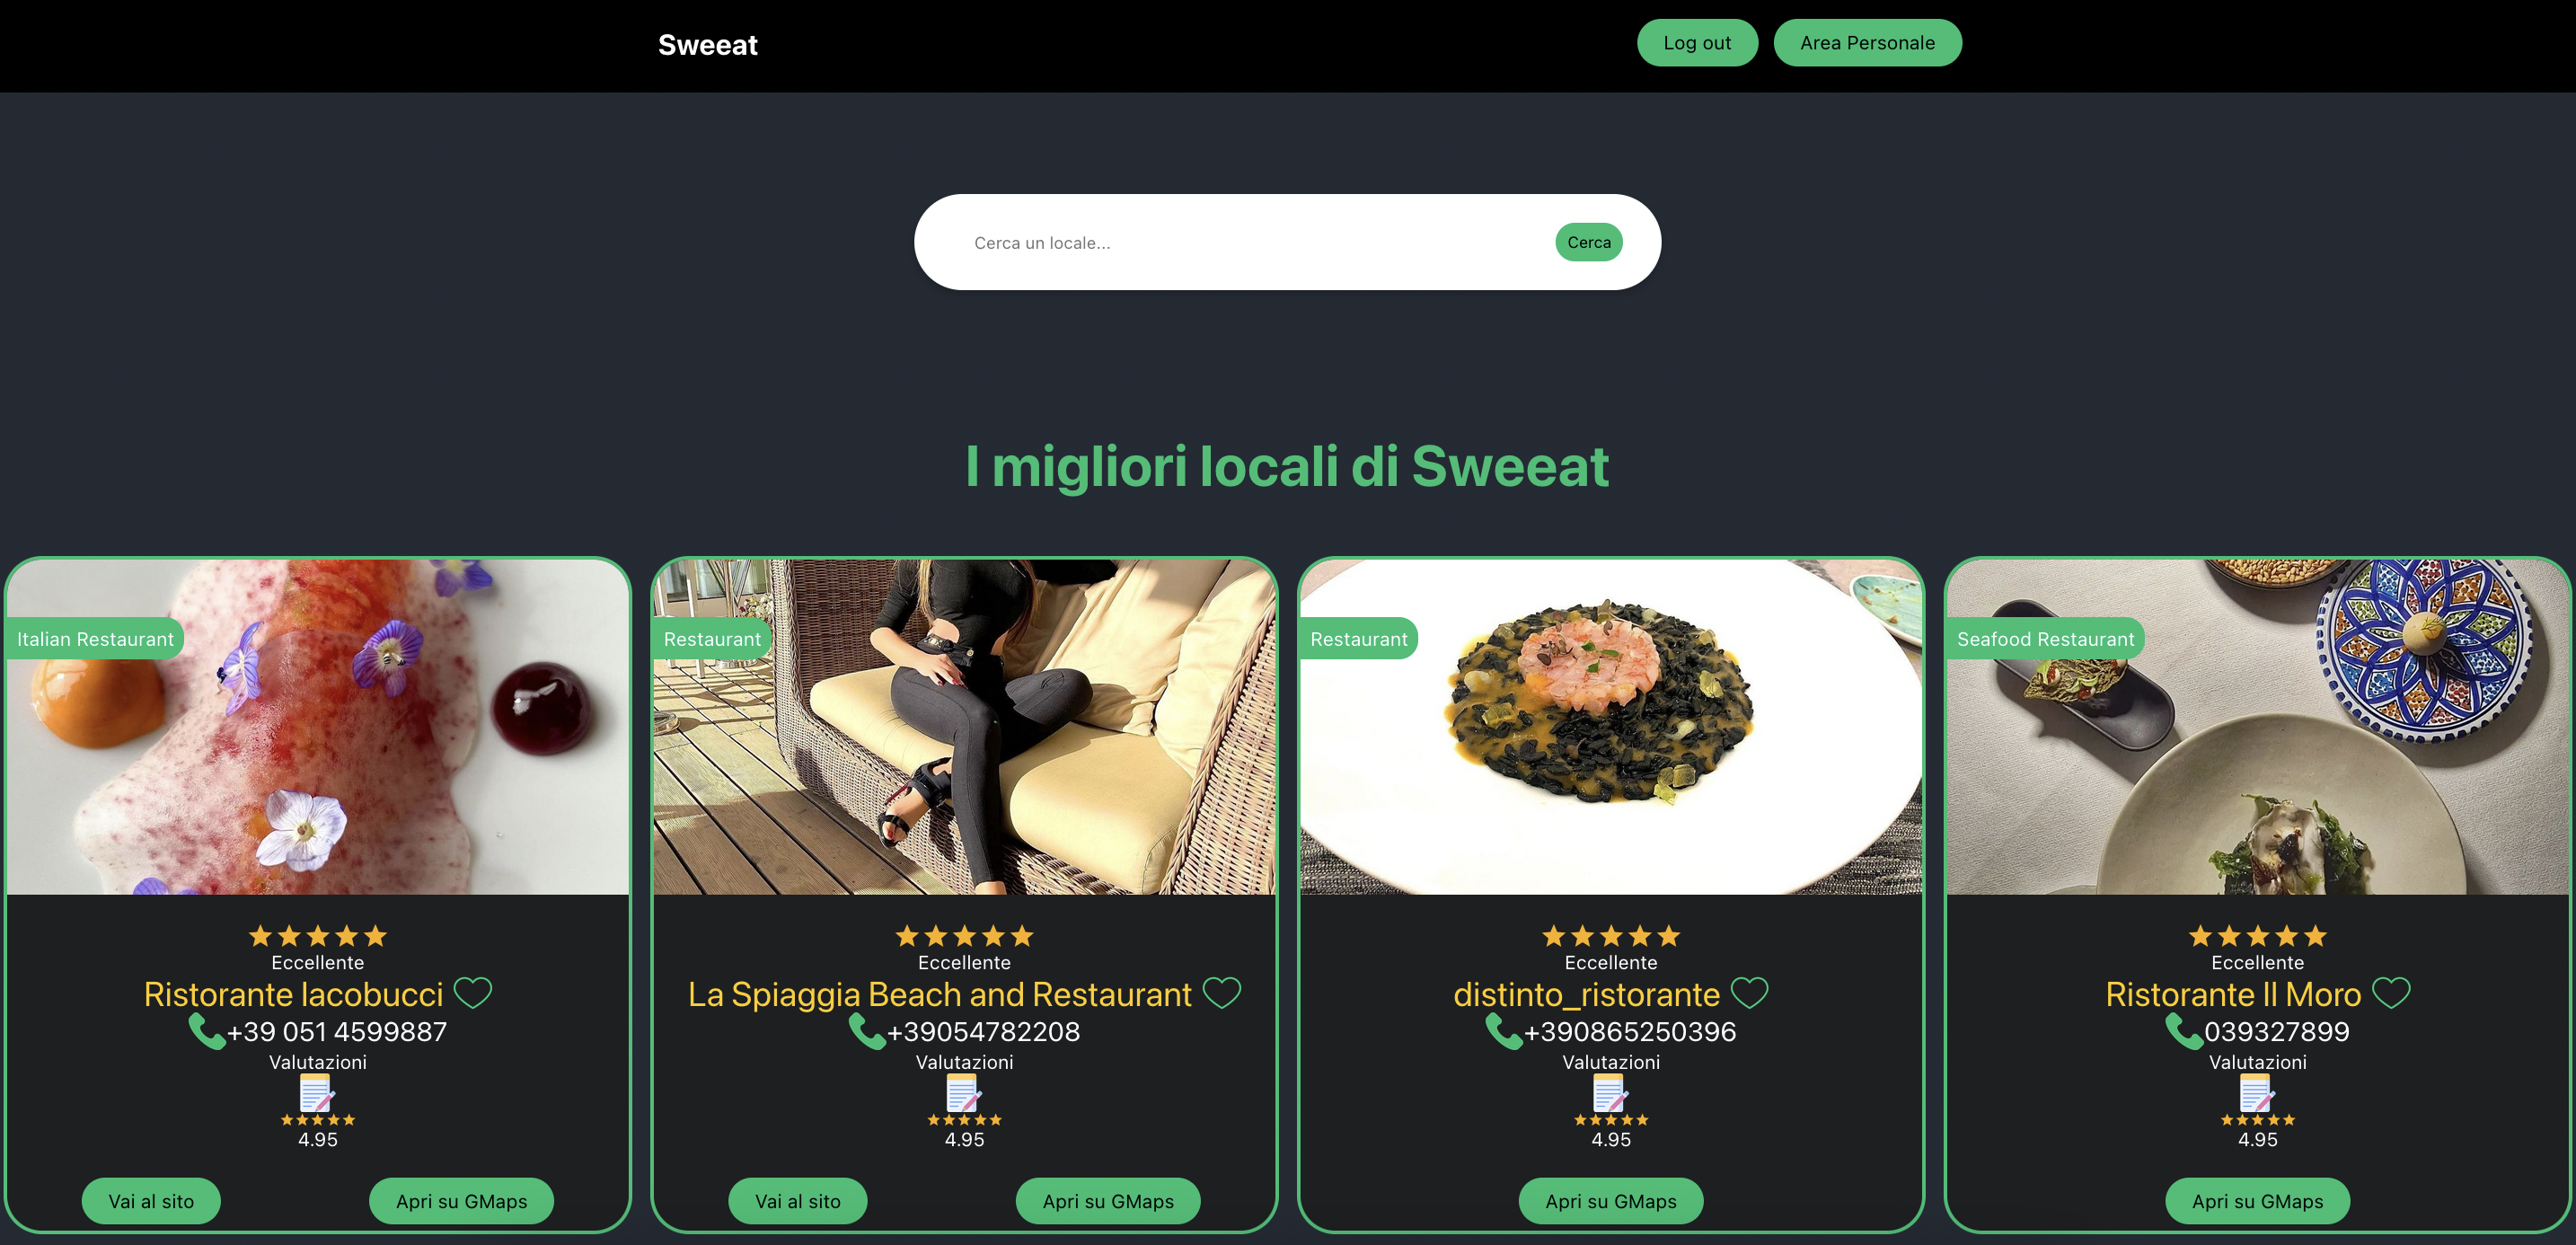
\includegraphics[scale=0.3]{./images/Homepage/Homepage.png} 
\caption{Homepage}
\end{figure}

\subsection{Ricerca}

Per effettuare una ricerca è necessario inserire il \textbf{nome del locale} cercato.

\begin{figure}[H]
\centering
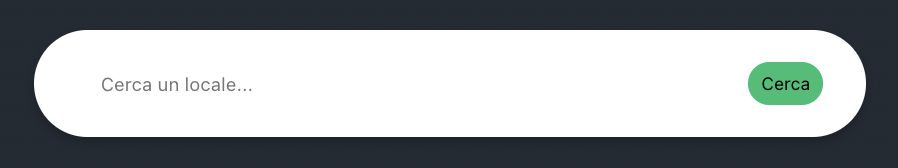
\includegraphics[scale=0.45]{./images/Homepage/Ricerca.png} 
\caption{Barra di ricerca nella Homepage}
\end{figure}

Quindi, va inserito il nome del locale da cercare e, per avviare la ricerca, è necessario cliccare su “\textbf{Cerca}”.

\begin{figure}[H]
\centering
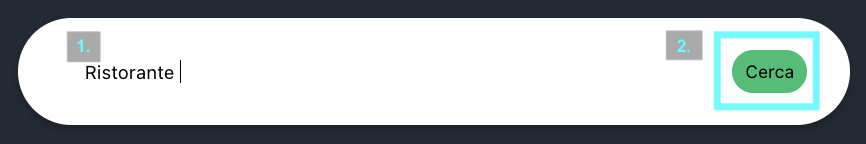
\includegraphics[scale=0.5]{./images/Homepage/Ricerca2.png} 
\caption{Inserimento dati ed avvio ricerca in Homepage}
\end{figure}

Una volta fatto ciò, verrà avviata la ricerca e l’utente verrà reindirizzato nella pagina dei risultati (\S{9}), la quale conterrà il risultato della ricerca (ossia, il locale cercato, dei locali alternativi o nessun locale).

\subsection{Visualizzare i migliori locali presenti su Sweeat}

Dalla pagina iniziale, oltre ad effettuare una ricerca, è possibile visualizzare i quattro migliori locali presenti nella piattaforma ed interagire con essi.

La sezione dedicata ai quattro migliori locali della piattaforma si trova sotto alla sezione contenente la barra di ricerca (sotto alla voce “I migliori locali di Sweeat”).

\begin{figure}[H]
\centering
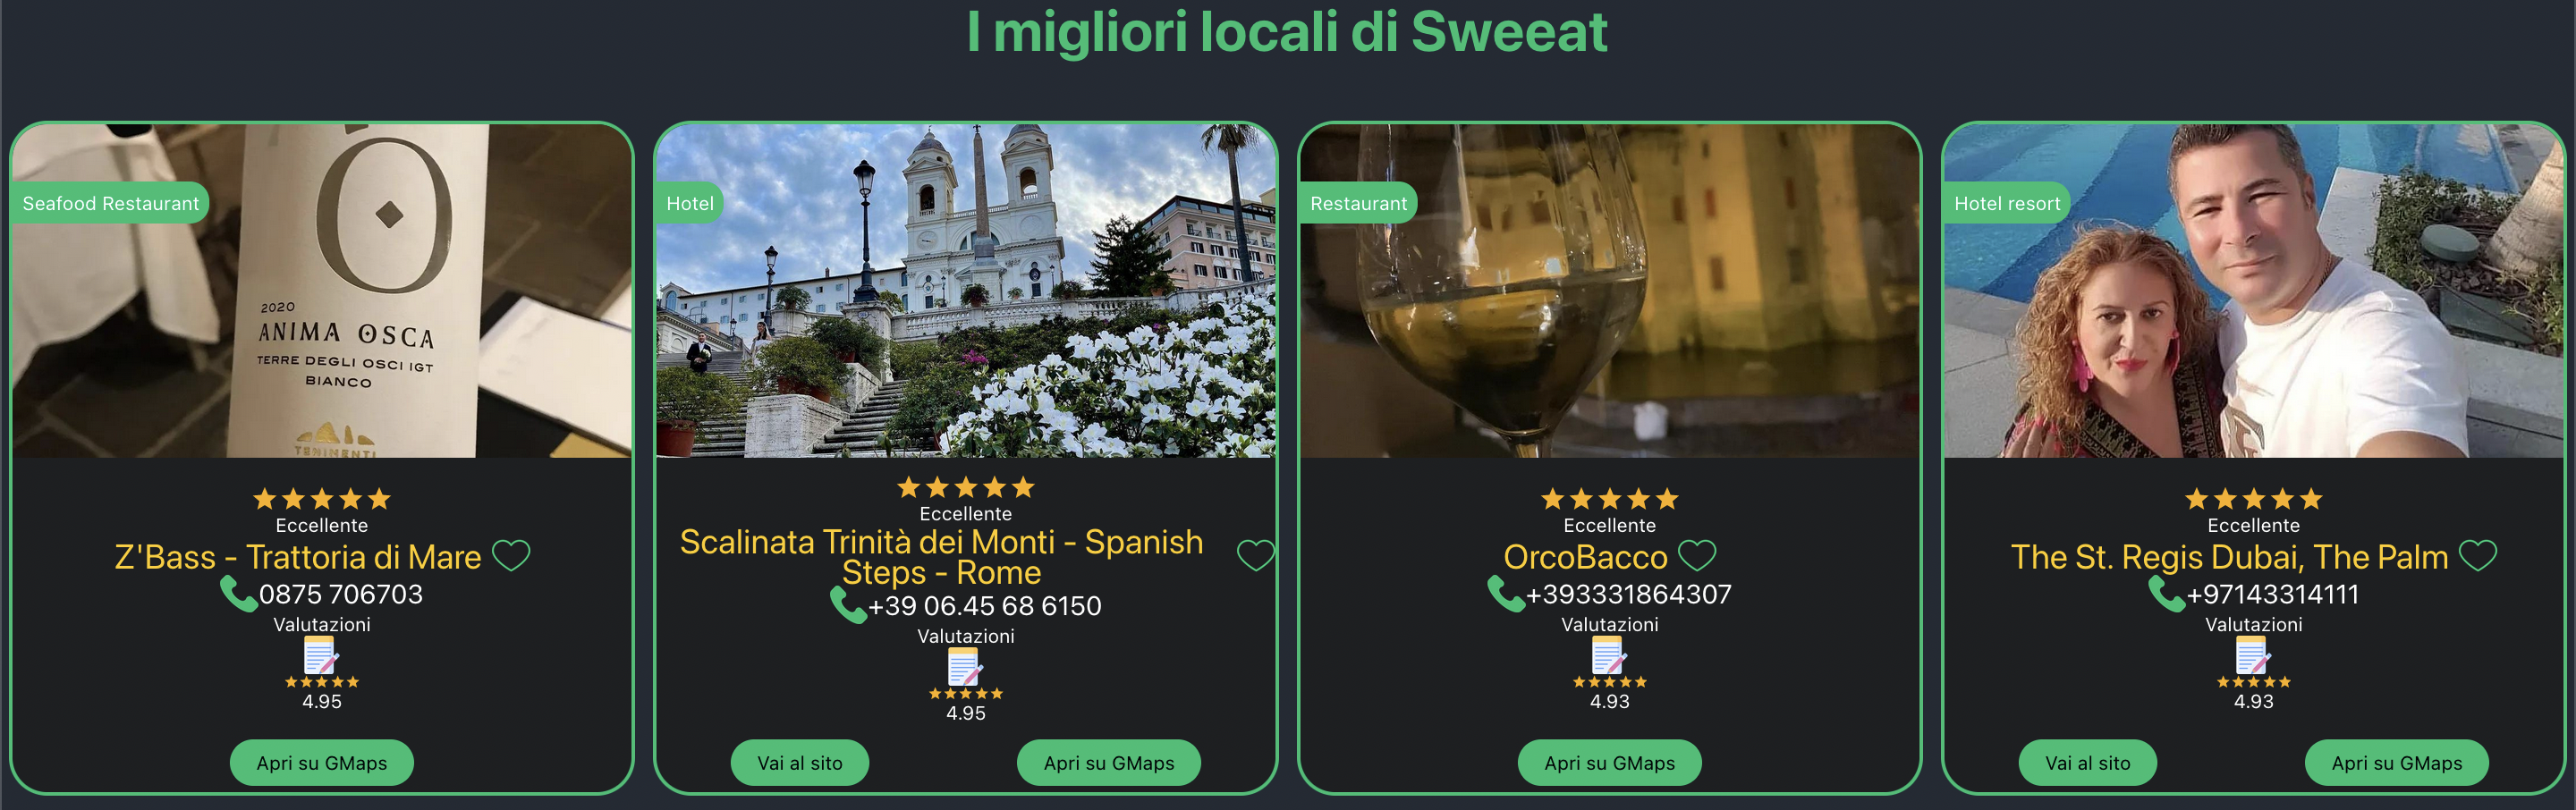
\includegraphics[scale=0.3]{./images/Homepage/MiglioriLocali.png} 
\caption{Inserimento dati ed avvio ricerca in Homepage}
\end{figure}

Per ciascun locale è possibile visualizzare le seguenti informazioni:

\begin{itemize}
\item Nome locale,
\item Valutazione complessiva,
\item Numero di telefono (opzionale),
\item Categoria,
\item Immagine di copertina,
\item Valutazione(*) per:
\begin{itemize}
\item Foto,
\item Testo,
\item Emoticons,
\end{itemize}
\item Link al sito web,
\item Link alla posizione del locale su Google Maps,
\item Possibilità di aggiungere o rimuovere il locale alla lista dei preferiti (funzionalità non ancora implementata).
\end{itemize}

\begin{figure}[H]
\centering
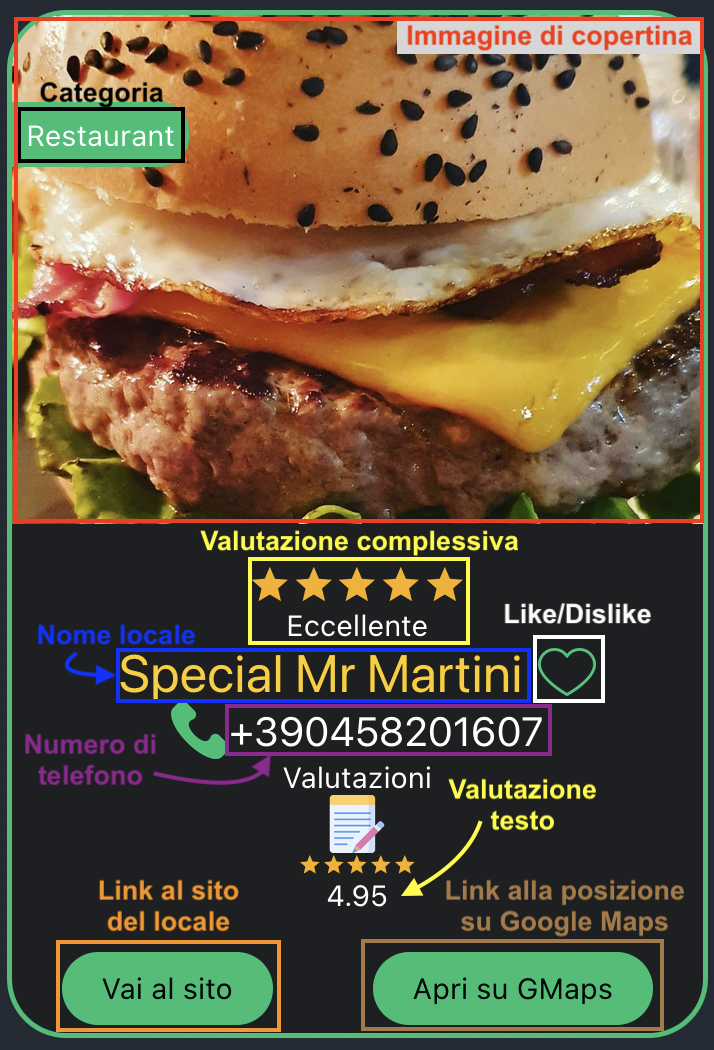
\includegraphics[scale=0.4]{./images/Homepage/Card.png} 
\caption{Card Locale in Homepage}
\end{figure}

(*) Per conoscere il significato delle valutazioni, consulta il paragrafo \S{9.2.1}. \\

La classifica dei migliori locali ha diverse pagine e per scorrerle è necessario cliccare su uno dei numeri presenti nella parte inferiore della pagina.

\begin{figure}[H]
\centering
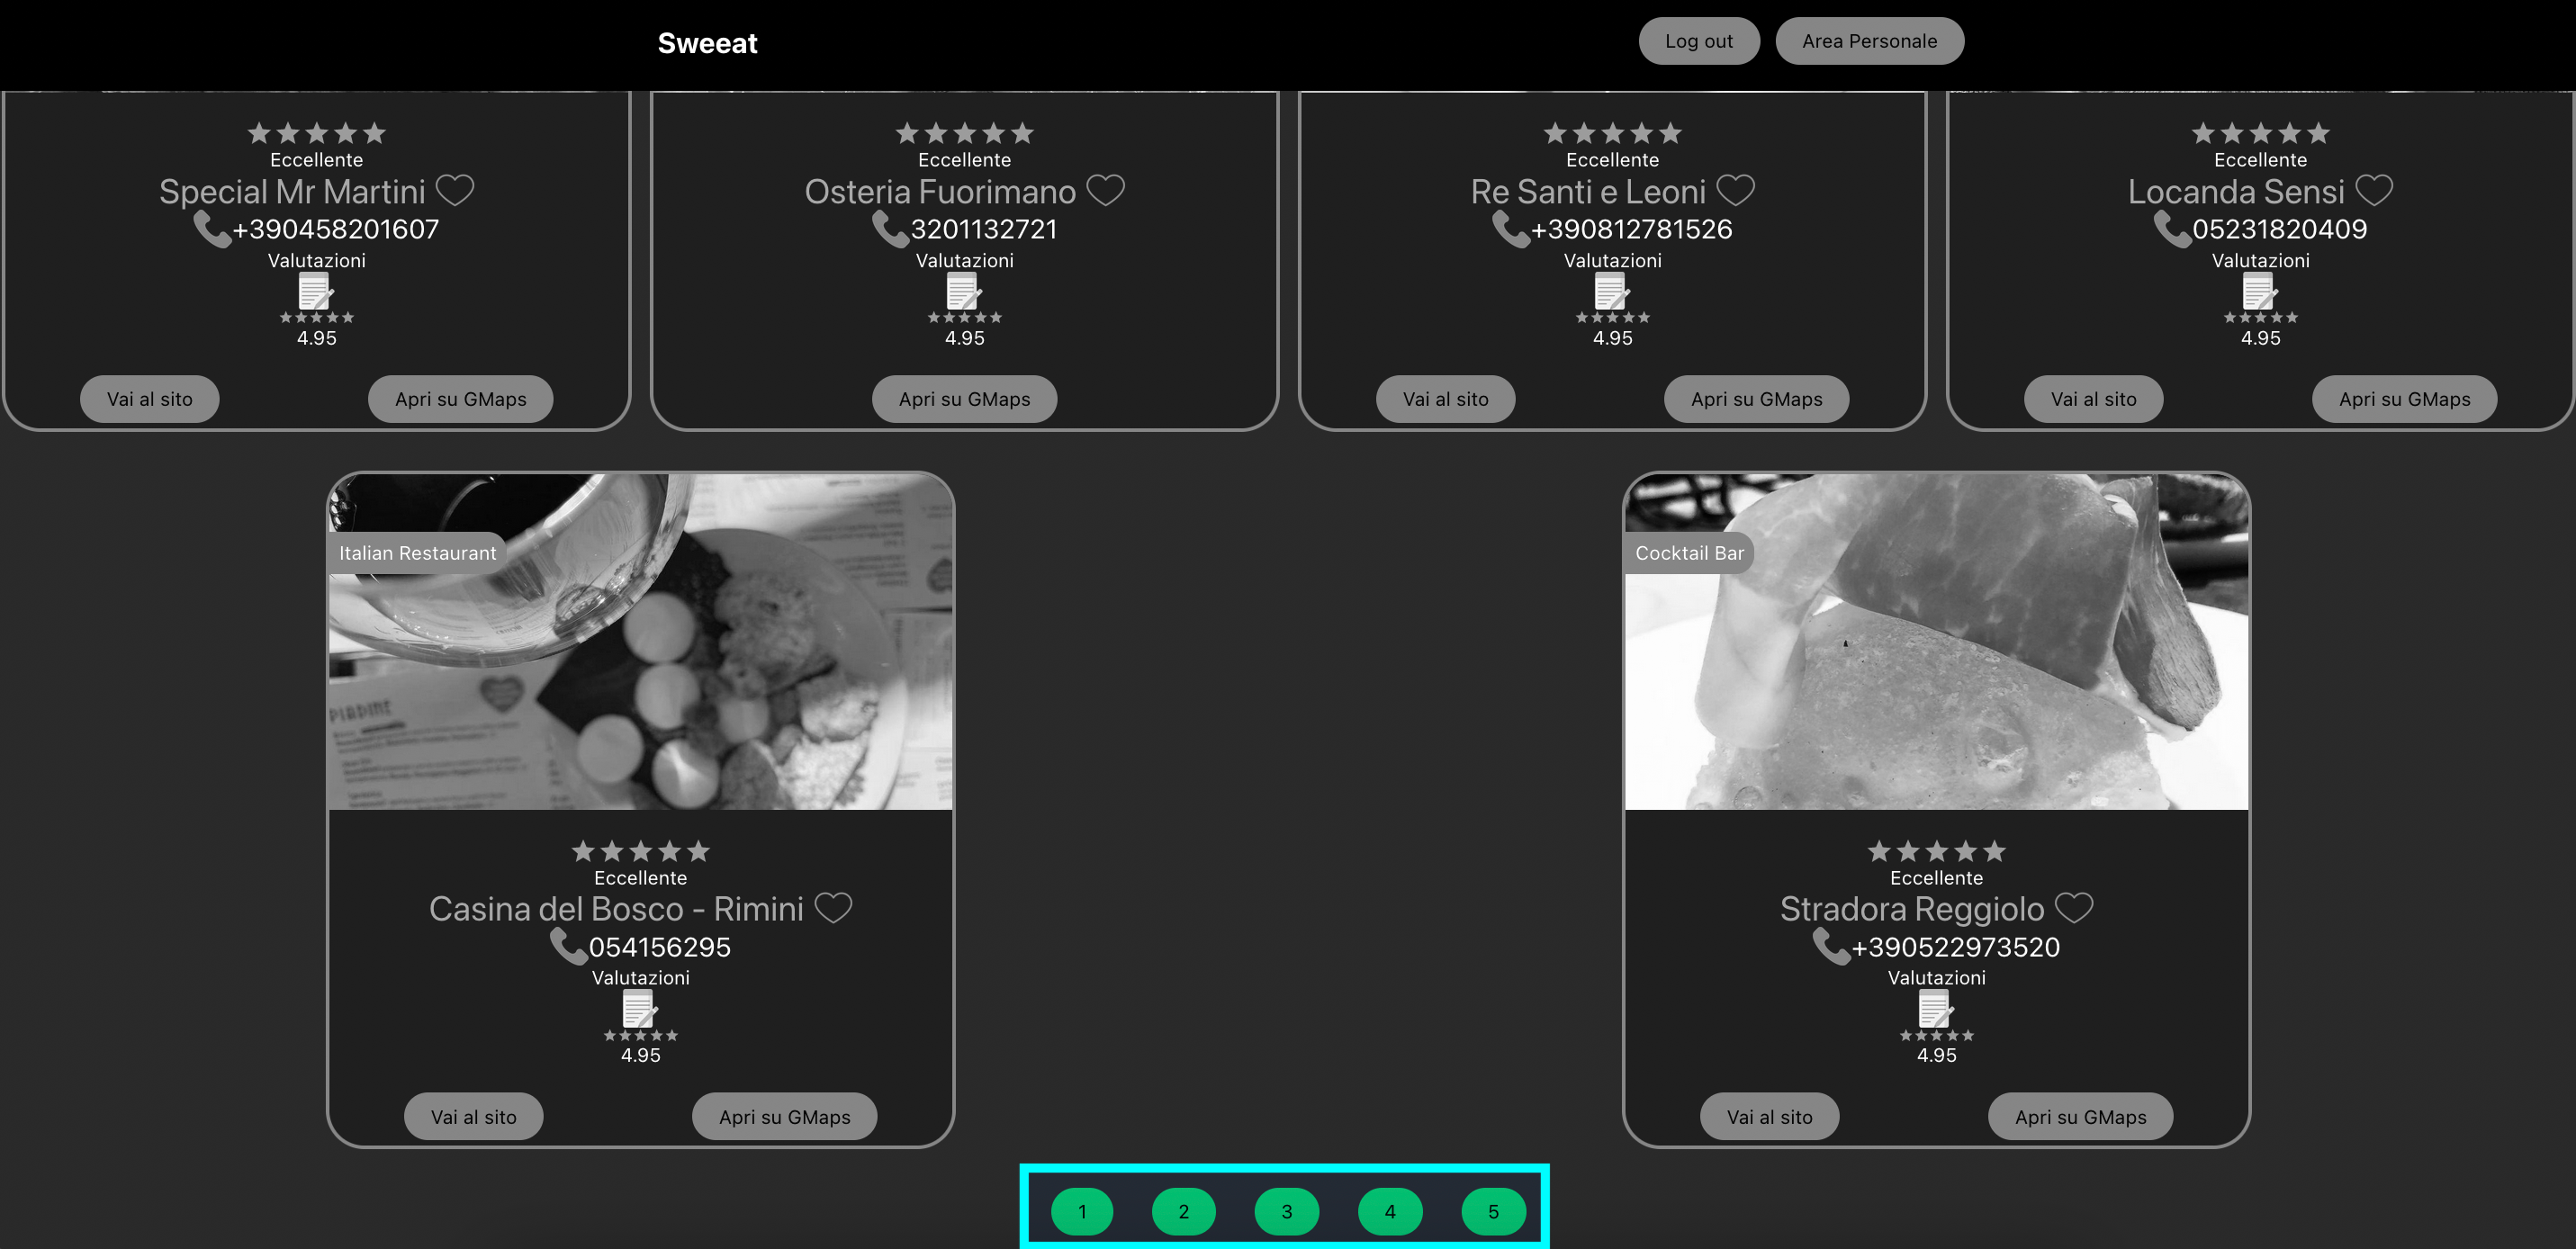
\includegraphics[scale=0.15]{./images/Homepage/Pagine.png} 
\caption{Visualizza altri migliori locali in Homepage}
\end{figure}

Inoltre, cliccando sul nome del locale all’utente verrà mostrata la \textbf{Pagina di dettaglio locale} (\S{10}) la quale, oltre al nome del locale e le informazioni di base appena descritte, conterrà i contenuti multimediali relativi a quel locale pubblicati su Instagram ed utilizzati per realizzare la WebApp.
